% (c) Gerard Baecker
\documentclass[fleqn,a4paper,12pt]{article}
  \usepackage[german]{babel}
  \usepackage[utf8]{inputenc}
  \usepackage{amsmath}    % Mathematische Symbole
  \usepackage{amssymb}     % Nochmehr mathematische Symbole
  \usepackage{dsfont}      % Schriftsatz fuer Zahlenmengensymbole
  %\usepackage{verbatim}   % erweiterte Verbatim-Umgebung
  \usepackage{alltt}       % Quasi-Verbatim-Umgebung
  \usepackage{fancyhdr}    % Eigene Kopfzeilen
  \usepackage{graphicx}    % Zum Einbinden von Grafiken
  % Einbinden einer eps-Grafik geht so: includegraphics{path}
  \usepackage{wrapfig}
  \usepackage{lscape}
  \usepackage{rotating}
  \usepackage{epstopdf}
  
  % Seitenraender
  \addtolength{\voffset}{-2cm}
  \addtolength{\textheight}{0cm}
  \addtolength{\hoffset}{0cm}
  \addtolength{\textwidth}{2cm}
  \addtolength{\headheight}{2cm} % fuer jeden Strichkode einen Zentimeter
  
  % Skalierung der Grafiken
  \setlength{\unitlength}{1cm}
  
  \pagestyle{fancy}            % Eigene Kopfzeilen verwenden
  \frenchspacing               % Kein Extrafreiraum nach Satzzeichen
  \setlength{\parindent}{0pt}  % Neue Absaetze nicht einruecken
  %\sloppy                     % Schlampige Absatzformatierung
  \fussy                       % Penible Absatzformatierung
  \linespread{1.5}             % Zeilenabstand
  
  % Font fuer Code 39
  \font\xlix=wlc39 scaled 1200
  \newcommand\barcode[1]{{\xlix@#1@}}
  
  % Name, Matrikelnummer, Barcode
  \newcommand\student[2]{
    \mbox{\scriptsize
    \begin{tabular}{@{}l@{}r@{}}
      \multicolumn{2}{@{}r@{}}{\barcode{#2}}\\
      #1&#2\\
    \end{tabular}}}
  
  % Kopfzeile
  \lhead{
    \small
    \textsc{Grundlagen der Signalverarbeitung \\
      WS 2017/2018 \\
      \"Ubung (\today)}
    \vfill}
  \rhead{
    \begin{tabular}[b]{@{}rr@{}}
      \student{Philipp Badenhoop}{572693} &
      \student{Steven Lange}{568733} \\
      \student{Pascal Jochmann}{575056} &
      \student{Kevin Trogant}{572451}
    \end{tabular}}
  
  \begin{document}
  "Ubungsaufgabe 7: \newline
  Aus der Dichtefunktion $p(x) = \lambda e^{-\lambda x}$, $x \geq 0$ ergibt sich die Verteilungsfunktion: \[F(x) = \int p(x) dx = -e^{-\lambda x} + C\]
  Für kontinuierliche Zufallsgrößen ergibt sich der gesuchte \textit{Median} $x_{med}$ folgendermaßen:
  \begin{align*}
      \int_{-\infty}^{x_{med}} p(x) dx &= \frac{1}{2} \\
      \Leftrightarrow \quad \int_0^{x_{med}} p(x) dx &= \frac{1}{2} \quad \text{Da }  p(x) = 0 \text{ für } x < 0 \\
      \Leftrightarrow \left[ -e^{-\lambda x} + C \right]_{0}^{x_{med}} &= \frac{1}{2} \\
      \text{Wähle } \lambda = \frac{1}{2} \\
      \Rightarrow \quad -e^{-\frac{1}{2}x_{med}} + 1 &= \frac{1}{2} \\
      \Rightarrow x_{med} = -2 \cdot \ln \frac{1}{2}
  \end{align*}
  Der Erwartungswert ergibt sich aus \[E(X) = \int_{-\infty}^{+\infty} x \cdot  p(x) dx\] \\
  Lösen des Integrals ergibt dann $E(X) = 2$. \\
  Die Varianz ergibt sich aus \[\textit{Var}(X) = \int_{-\infty}^{+\infty} ( x - E(X) )^2 \cdot p(x) dx\]
  Lösen des Integrals ergibt dann $\textit{Var}(X) = 4$.
  \begin{figure}
      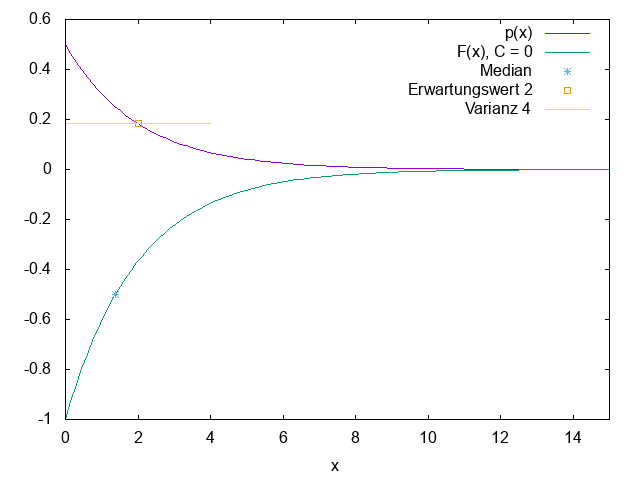
\includegraphics[width=1.0\textwidth]{sv0_7.png}
      \caption{(7) Darstellung der gegebenen Dichtefunktion und einiger Kenngrößen}
  \end{figure}
  \newpage
  "Ubungsaufgabe 9: \newline
  \begin{sidewaysfigure}
      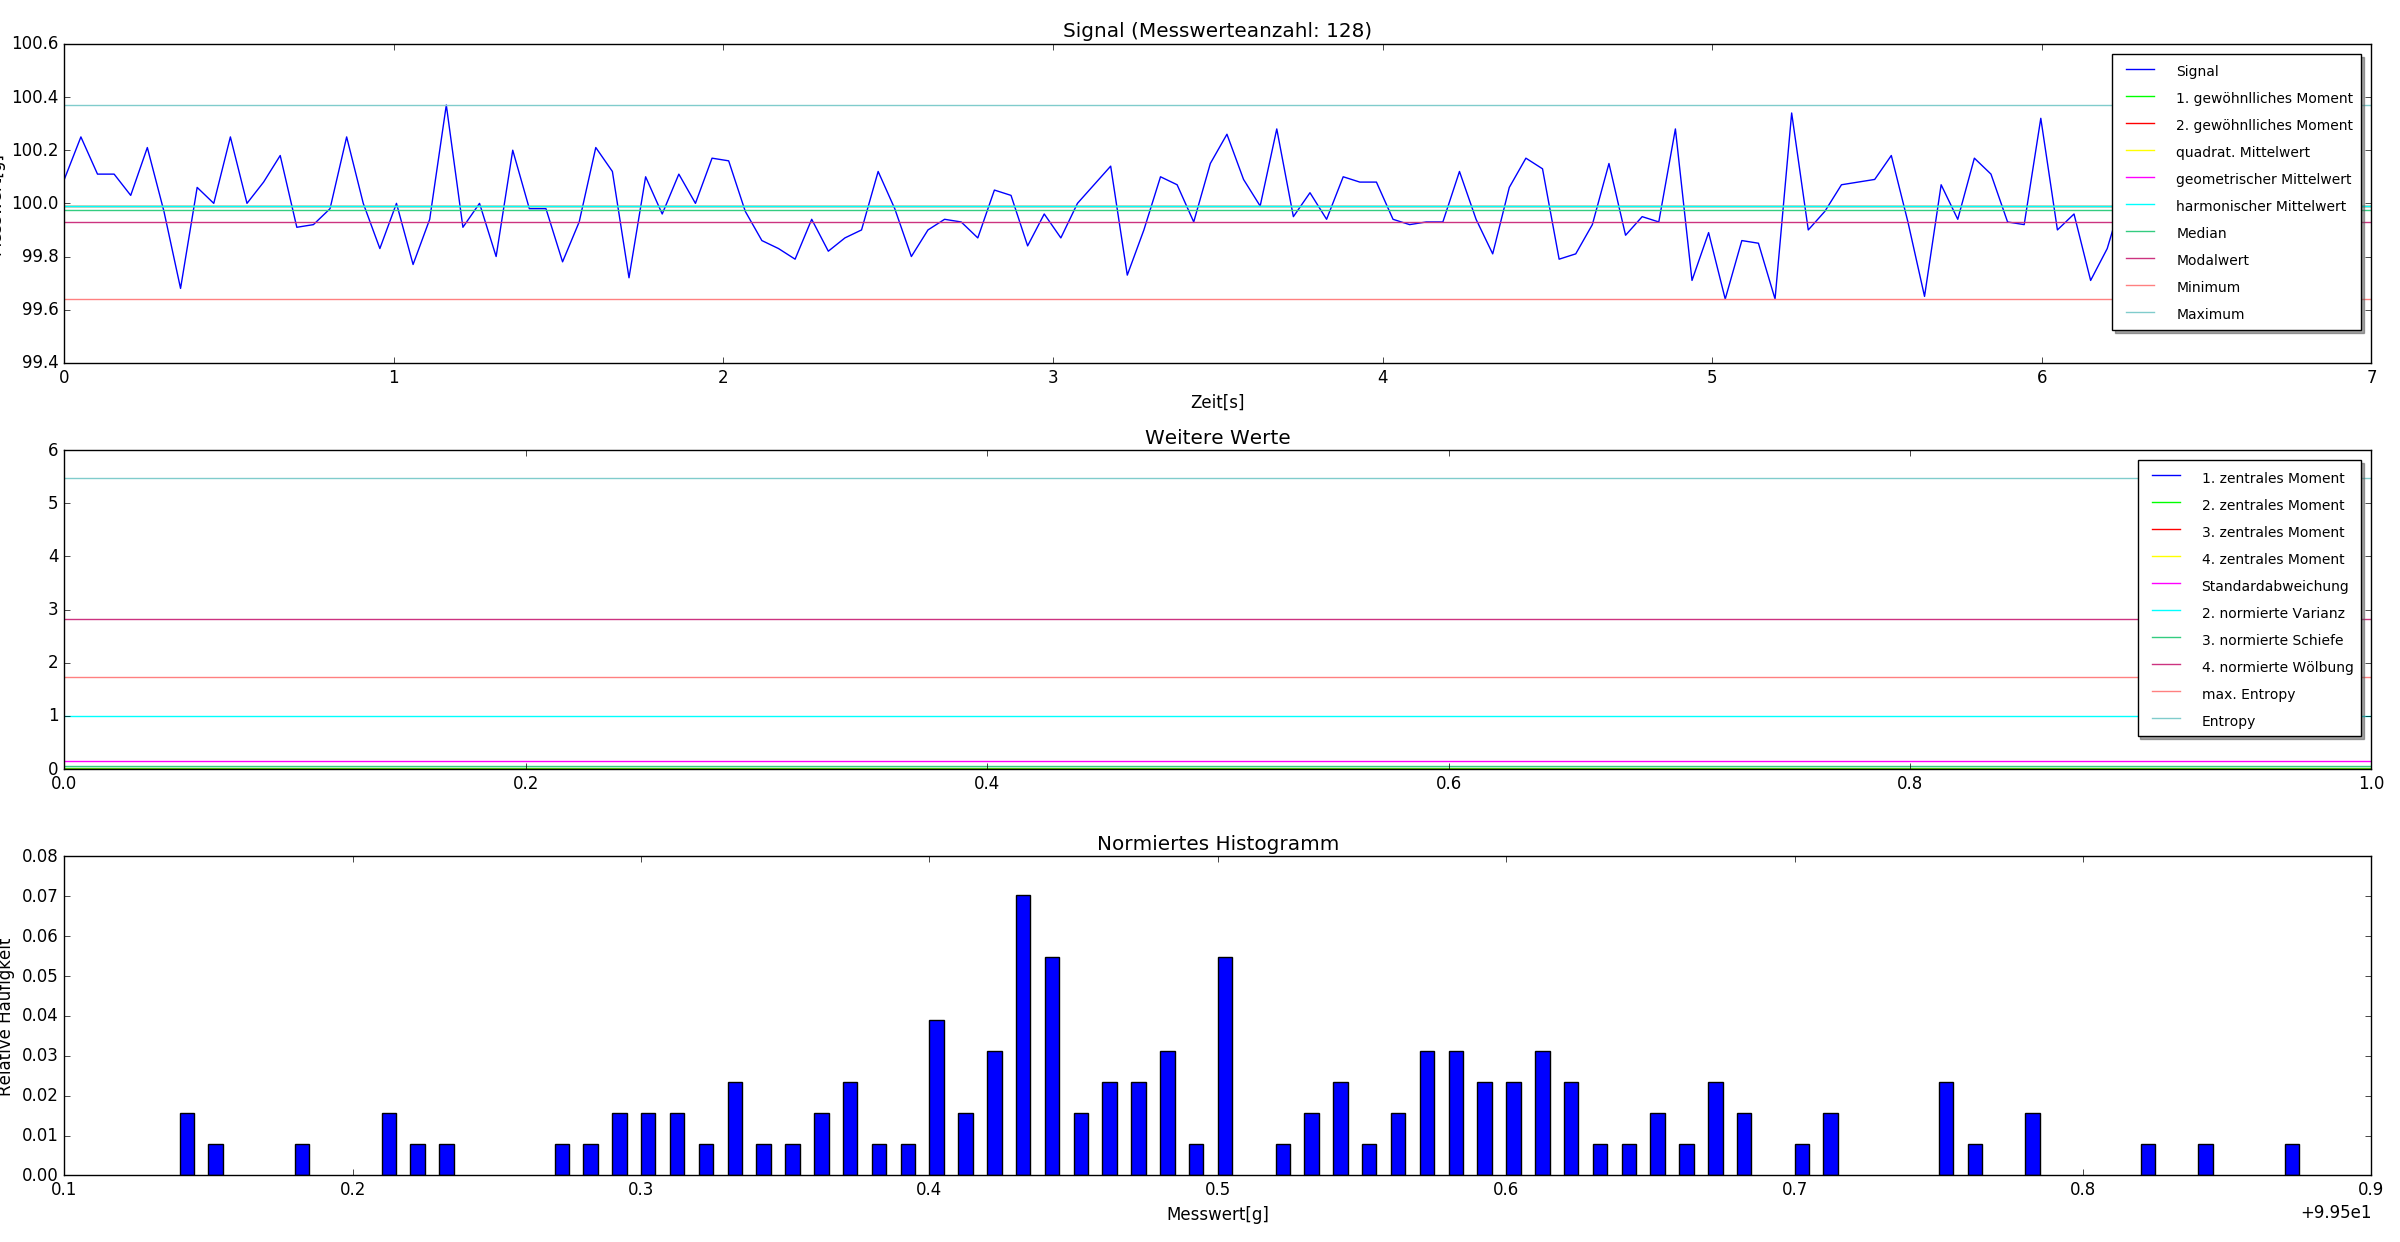
\includegraphics[width=1.0\textwidth]{a9_128.png}
      \caption{(9) Messreihe mit 128 Messwerten}
  \end{sidewaysfigure}
  \begin{sidewaysfigure}
    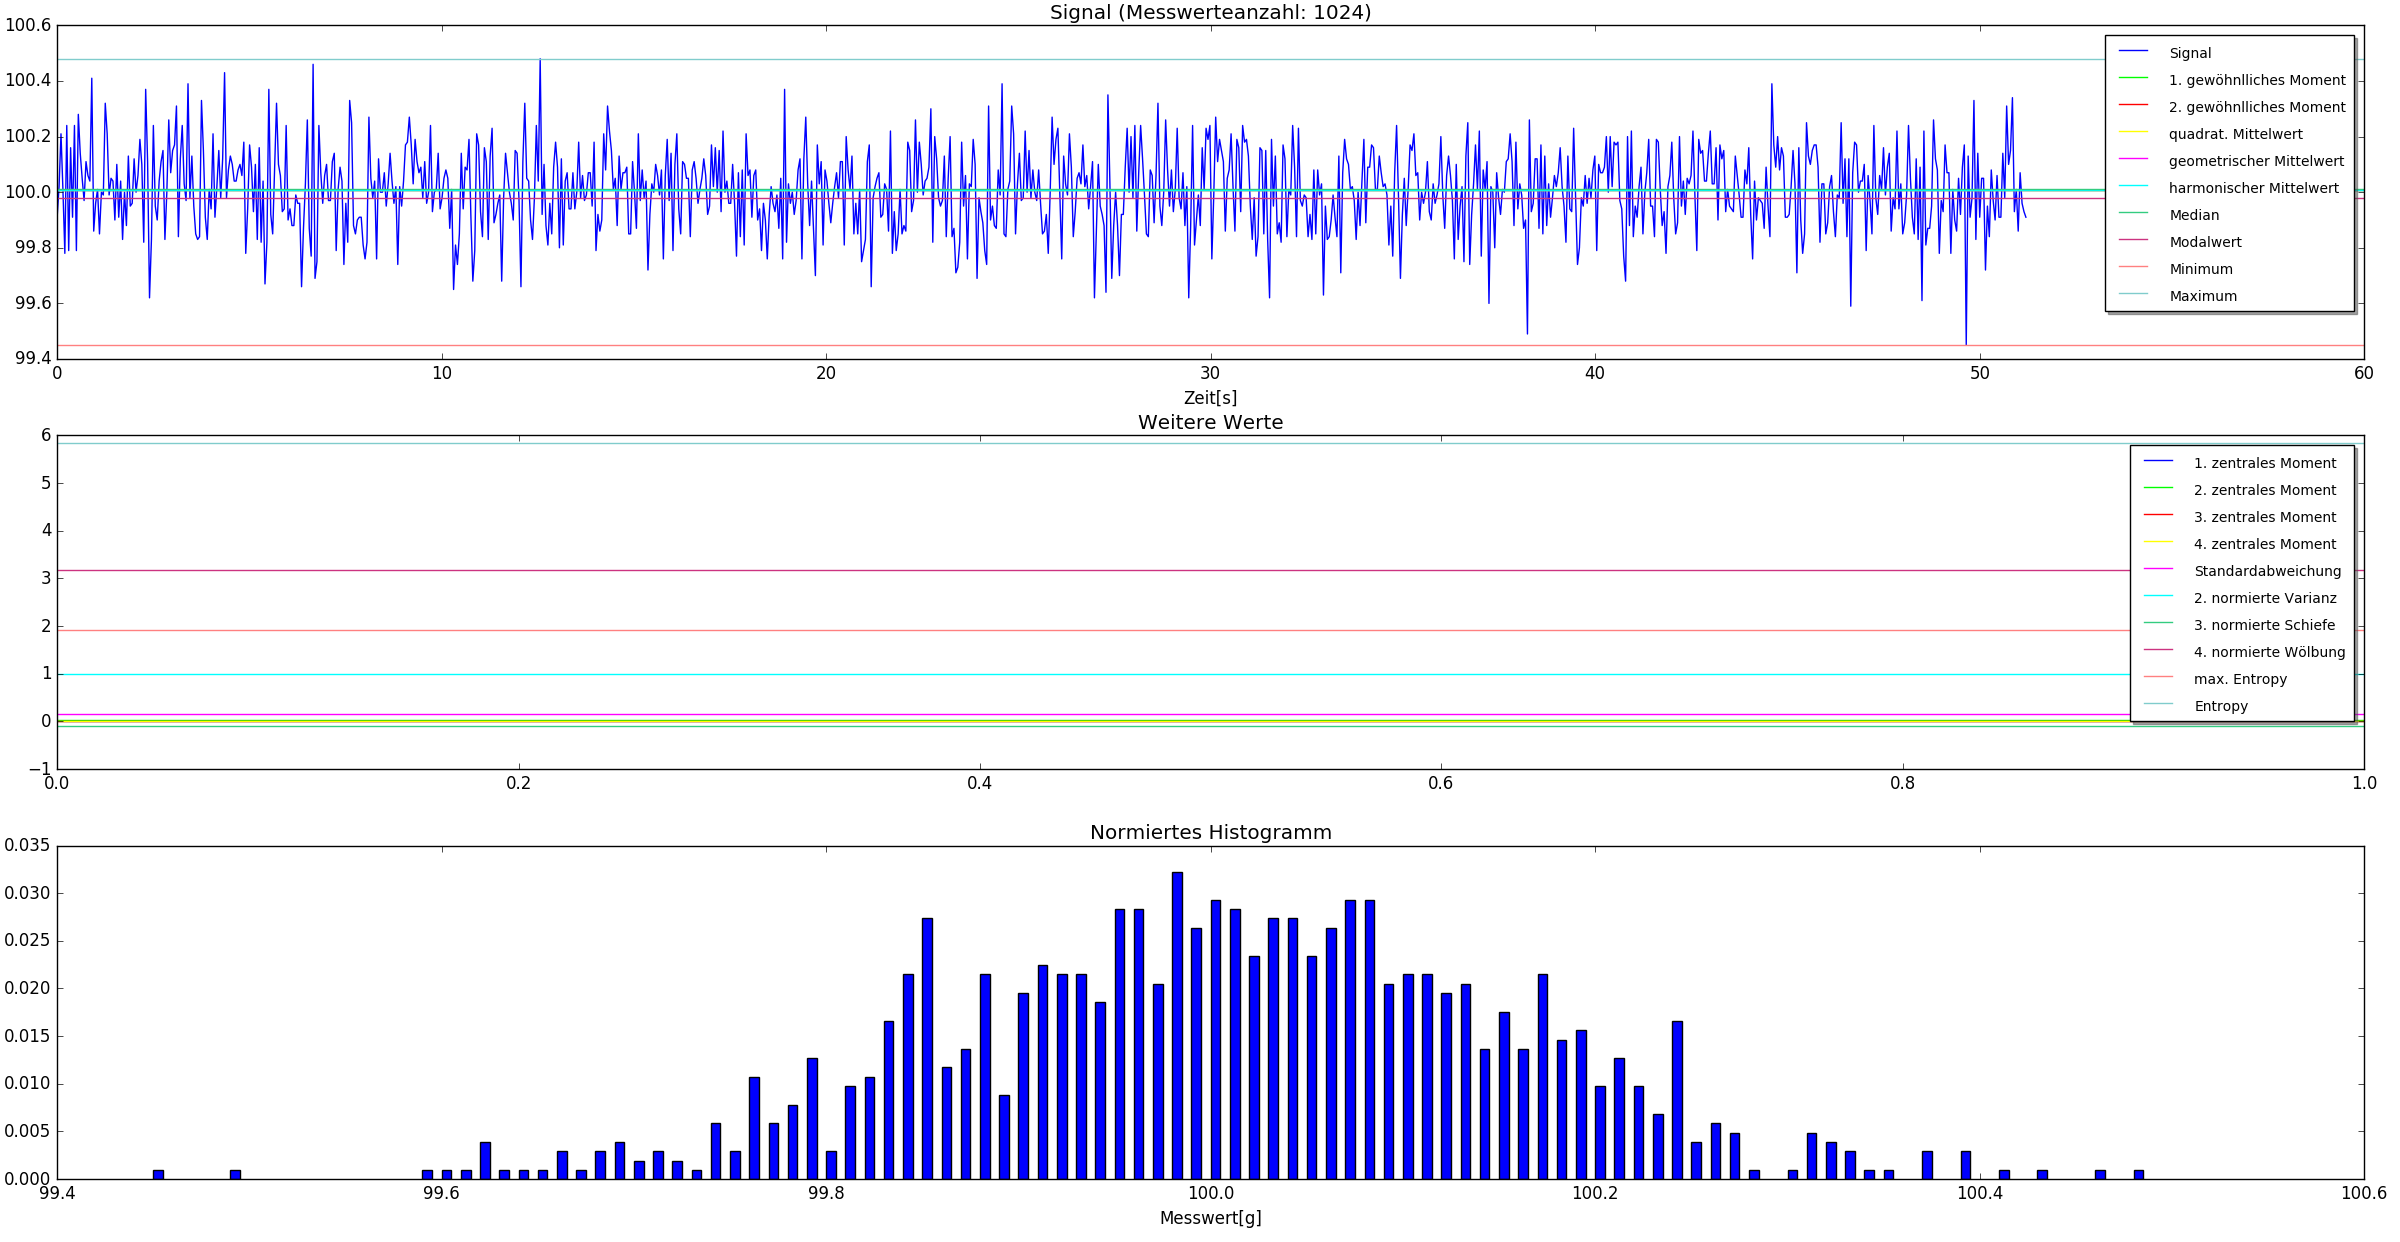
\includegraphics[width=1.0\textwidth]{a9_1024.png}
    \caption{(9) Messreihe mit 1024 Messwerten}
  \end{sidewaysfigure}
  Zur Messreihe mit 1024 Messwerten: \newline
  Mittelungleichung von Cauchy erfüllt: ja \newline
  Normalverteilt: ja \newline
  Interpretation Entropie: Der mittlere Informationsgehalt (Entropie) liegt mit $\approx 5.9$ relativ nah am maximalen Informationsgehalt $\approx 6.4$ (max. Entropie).
  Damit ist der Informationsgehalt eines Messwertes relativ groß. \newpage

  "Ubungsaufgabe 10: \newline
  \begin{sidewaysfigure}
    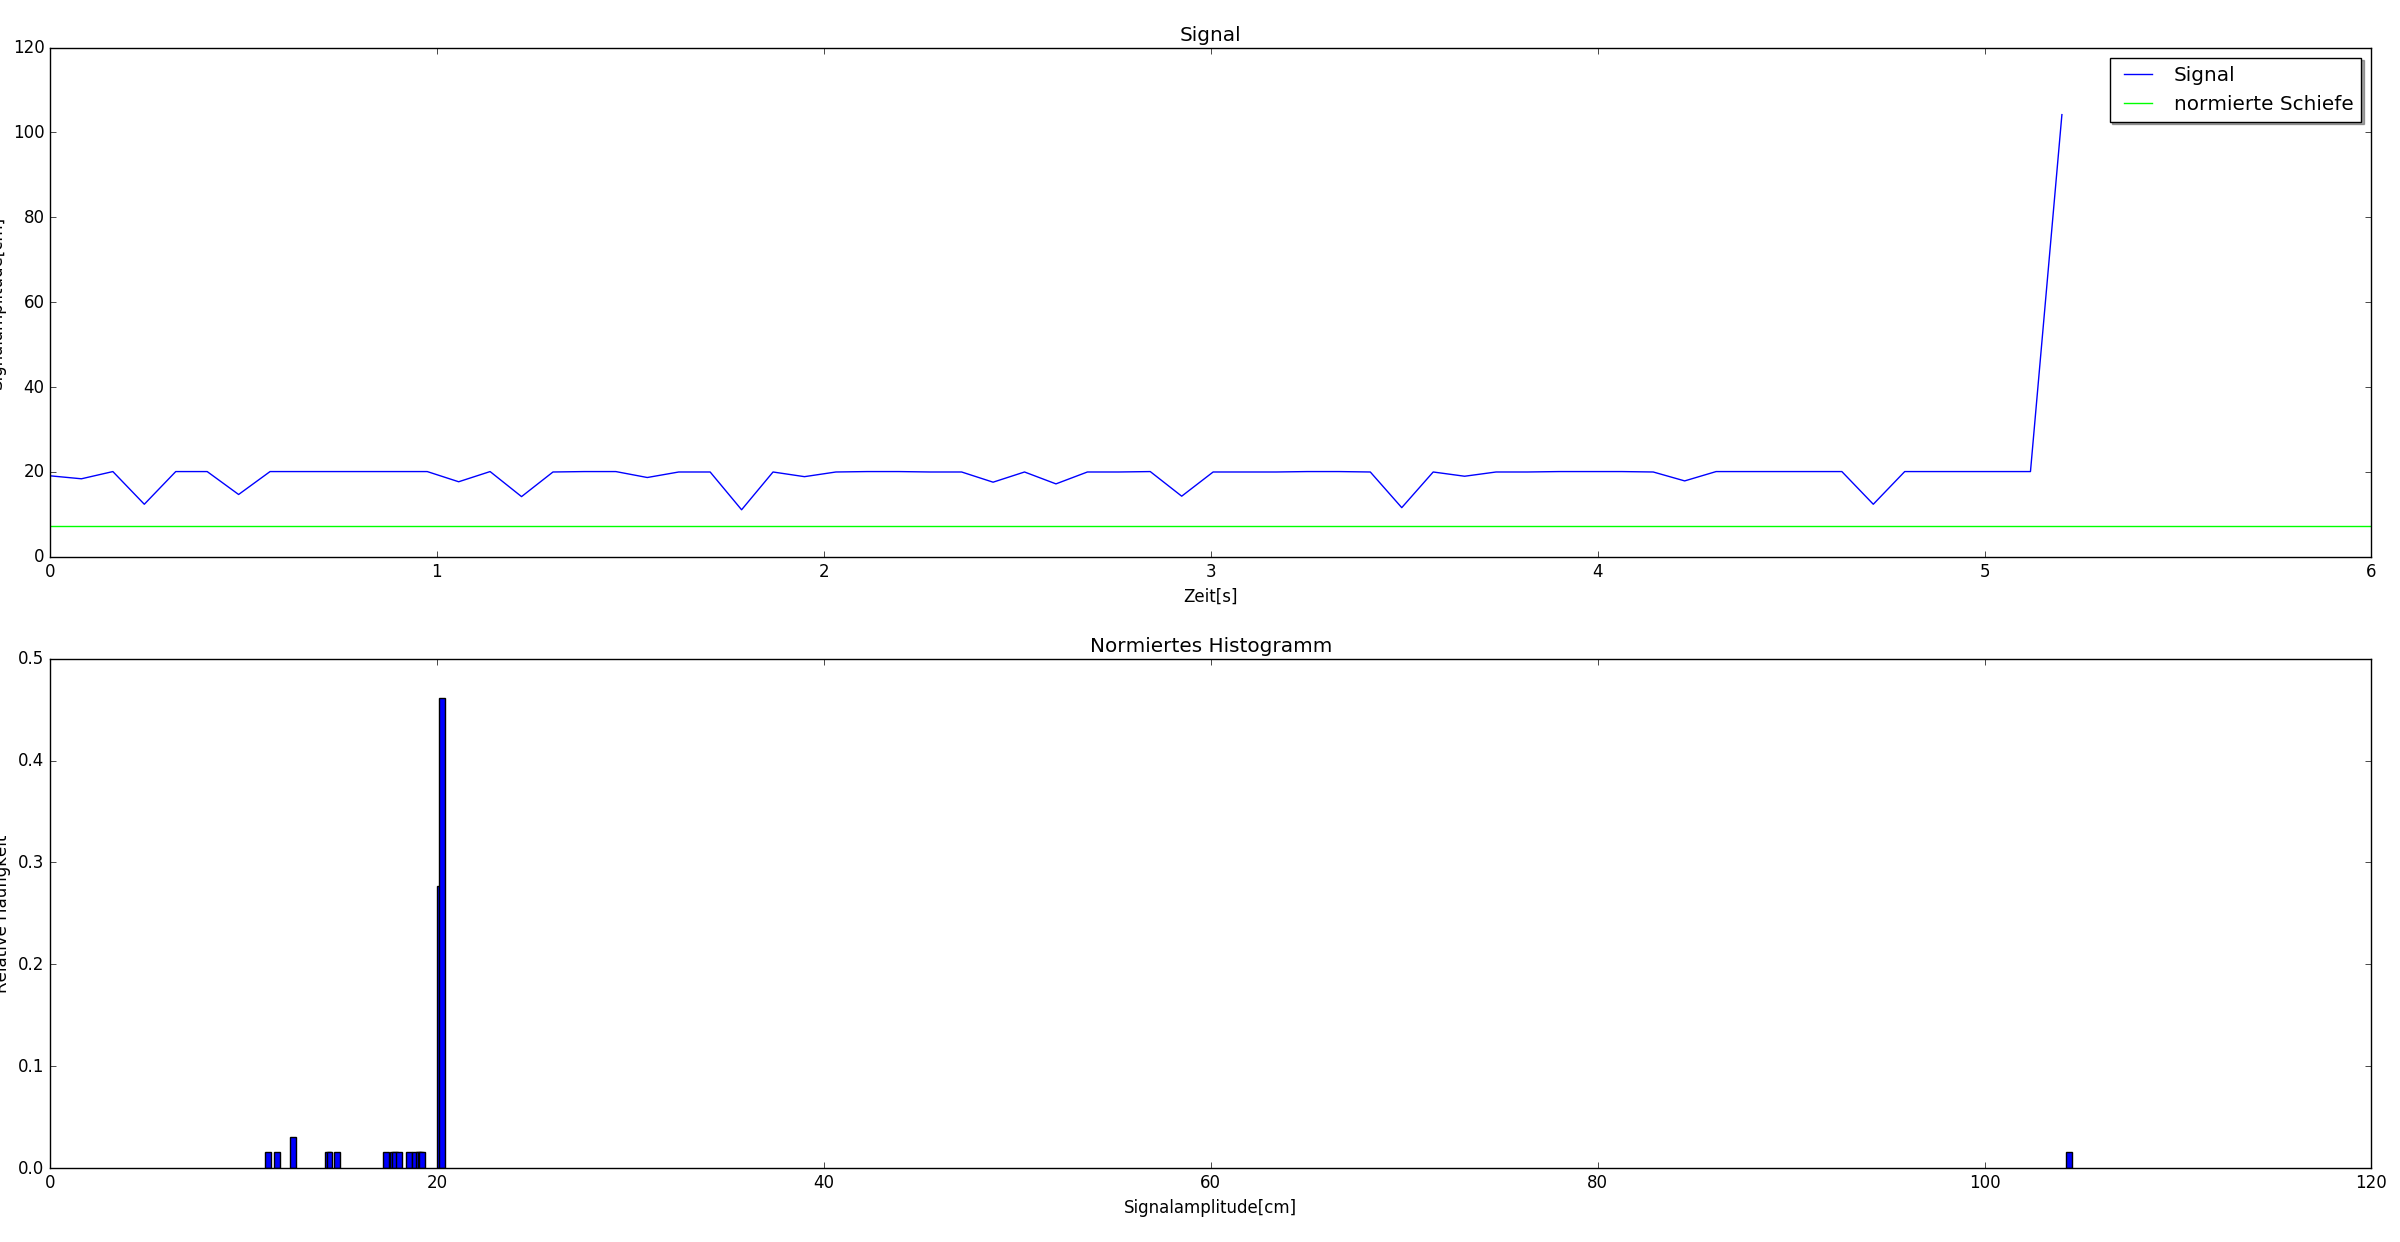
\includegraphics[width=1.0\textwidth]{a10.png}
    \caption{(10) Chaospendelprozess}
  \end{sidewaysfigure}
  Normierte Schiefe $\approx 7.32$ \newline
  Anmerkung: Hier scheint irgendetwas mit der Website schief zu laufen, da obwohl 128 Messwerte angefordert werden, nur 65 angezeigt werden.
  Außerdem sieht der Prozess nicht nach einem Chaospendel aus.

  \end{document}
  